% =============================================================================
% 05-queues-notes.tex — Lecture Notes for Week 5:
% First In, First Out (Queues, Circular Buffers, Deques, and Priority)
%
% DERIVED ARTIFACT. Source of truth: Slides/CS301/05-queues.tex
% (29 frames/38 pages, compiled clean).
% Generated by /lecture-notes at the "textbook-candidate prose" Detail Bar
% (every trace step written out, every example fully solved, Exercises with a
% separate Solutions block, reading guidance per section); do not hand-edit
% content independently of the Beamer source without re-running /qa-notes
% afterward (single-source-of-truth.md).
%
% Page-grounding (inherited 1:1 from the deck header; no upgrades):
%   Karumanchi2017 Ch.5 (Queues, pp.205-223 PDF: Queue ADT and variants) and
%     Ch.7 (pp.369-408 PDF: Priority Queue ADT); Sedgewick2011 Sec.1.3 p.120
%     (queue as a collection ADT) and Sec.2.4 p.308 (priority queues).
%     Horowitz & Sahni Ch.3 / Aho-Hopcroft-Ullman Ch.2 at chapter level only
%     (not page-indexed).
%   Socratic "Check Your Prediction" frames and the three "Before You Go"
%   predictions are folded into the prose as worked checks with the deck's
%   own answers; the Week 6 (linked lists), Week 7 (list-based queue), Week 11
%   (heaps), and Week 12 (BFS frontier) forward pointers are preserved as stated.
%
% Compile with (Windows/MiKTeX, ';'-joined TEXINPUTS/BIBINPUTS): cd Notes/CS301 &&
%   $env:TEXINPUTS="../../Preambles;"; xelatex -interaction=nonstopmode 05-queues-notes.tex
%   $env:BIBINPUTS="../..;"; bibtex 05-queues-notes
%   $env:TEXINPUTS="../../Preambles;"; xelatex -interaction=nonstopmode 05-queues-notes.tex  (x2)
% =============================================================================

\documentclass[11pt]{article}
\usepackage[margin=1in]{geometry}
% =============================================================================
% Preambles/header.tex — shared LaTeX/Beamer preamble for this project
%
% Use from a Beamer lecture by prepending:
%     \input{header}
% and compiling with TEXINPUTS=../Preambles:$TEXINPUTS (the /compile-latex
% skill does this automatically).
%
% PALETTE CONTRACT. Color names defined here MUST match the names in
% Quarto/theme-template.scss so Beamer and Quarto renderings use the same
% palette. The scripts/check-palette-sync.sh script enforces this.
%
% To customize: edit the HEX values below AND the matching $variable in
% Quarto/theme-template.scss, then run scripts/check-palette-sync.sh.
% =============================================================================

% -----------------------------------------------------------------------------
% Engine detection + encoding
%
% Our /compile-latex skill uses XeLaTeX, where inputenc is unnecessary and
% can produce encoding warnings. Only load inputenc under pdfTeX.
% -----------------------------------------------------------------------------
\usepackage{iftex}
\ifPDFTeX
  \usepackage[utf8]{inputenc}
\fi

\usepackage{amsmath, amssymb, amsthm}
\usepackage{booktabs}
\usepackage{graphicx}

% -----------------------------------------------------------------------------
% PALETTE — mirrors Quarto/theme-template.scss variable names.
% Load xcolor and define colors BEFORE anything that references them
% (notably hyperref, hypersetup, and the Beamer color assignments).
% -----------------------------------------------------------------------------
\usepackage{xcolor}

\definecolor{primary-blue}{HTML}{012169}      % headings, accents
\definecolor{primary-gold}{HTML}{B9975B}      % emphasis, borders
\definecolor{highlight-yellow}{HTML}{F2A900}  % markers, alerts
\definecolor{light-bg}{HTML}{E8EDF5}          % title / section backgrounds
\definecolor{jet}{HTML}{1A1A1A}               % body text

% Semantic colors (used in diagrams and annotations)
\definecolor{positive}{HTML}{15803D}          % good / observed / identified
\definecolor{negative}{HTML}{B91C1C}          % bad / problematic / bias
\definecolor{neutral}{HTML}{525252}           % reference / context

% Highlight accents (match .hi-* classes in the SCSS)
\definecolor{hi-slate}{HTML}{314F4F}
\definecolor{hi-green}{HTML}{2E8B57}
\definecolor{hi-red}{HTML}{C41E3A}

% Semantic aliases so skill templates and snippets can write
% \textcolor{accent}{...} without hard-coding "primary-blue".
\colorlet{accent}{primary-blue}
\colorlet{accent2}{primary-gold}

% -----------------------------------------------------------------------------
% Hyperref — loaded AFTER xcolor + palette so link colors resolve.
% -----------------------------------------------------------------------------
\usepackage{hyperref}
\hypersetup{colorlinks=true, linkcolor=primary-blue, urlcolor=primary-blue,
            citecolor=primary-blue, pdfborder={0 0 0}}

% -----------------------------------------------------------------------------
% Course code — set once per deck (after \input{header}, before \begin{document})
% via \coursecode{CS401}. Shown in the footer on every slide so a deck's course
% is identifiable without opening the title page. Empty by default.
% -----------------------------------------------------------------------------
\makeatletter
\newcommand{\coursecode}[1]{\gdef\@coursecodetext{#1}}
\gdef\@coursecodetext{}
\makeatother

% -----------------------------------------------------------------------------
% Beamer theme assignments (only apply under Beamer).
%
% We detect Beamer via \@ifclassloaded{beamer}, which is the documented,
% non-internal way. This must be wrapped in \makeatletter/\makeatother
% because \@ifclassloaded contains an @-catcode character.
% -----------------------------------------------------------------------------
\makeatletter
\@ifclassloaded{beamer}{%
  \usefonttheme{professionalfonts}
  \setbeamercolor{structure}{fg=primary-blue}
  \setbeamercolor{frametitle}{fg=primary-blue}
  \setbeamercolor{title}{fg=primary-blue}
  \setbeamercolor{subtitle}{fg=primary-gold}
  \setbeamercolor{author}{fg=primary-blue}
  \setbeamercolor{institute}{fg=neutral}
  \setbeamercolor{date}{fg=primary-gold}
  \setbeamercolor{itemize item}{fg=primary-blue}
  \setbeamercolor{itemize subitem}{fg=primary-gold}
  \setbeamercolor{alerted text}{fg=primary-gold}
  \setbeamercolor{block title}{fg=white, bg=primary-blue}
  \setbeamercolor{block body}{bg=light-bg}
  % Semantic block variants: block=definition/concept (blue), exampleblock=
  % worked example (green/positive), alertblock=key takeaway or caution (gold).
  % Keep to <=2 colored boxes per slide across ALL three variants (INV-7).
  \setbeamercolor{block title example}{fg=white, bg=positive}
  \setbeamercolor{block body example}{bg=light-bg}
  \setbeamercolor{block title alerted}{fg=white, bg=primary-gold}
  \setbeamercolor{block body alerted}{bg=light-bg}

  % Minimal footer: course code (left) + page X / N (right), no navigation clutter
  \setbeamertemplate{navigation symbols}{}
  \setbeamertemplate{footline}{%
    \color{neutral}\footnotesize\hspace{0.7em}\@coursecodetext\hfill
    \insertframenumber/\inserttotalframenumber\hspace{0.7em}\vspace{0.3em}}
}{}
\makeatother

% -----------------------------------------------------------------------------
% TikZ setup — libraries the snippet gallery uses
% -----------------------------------------------------------------------------
\usepackage{tikz}
\usetikzlibrary{arrows.meta, positioning, calc, decorations.pathreplacing,
                fit, shapes.geometric, backgrounds}

% Shared TikZ styles — snippets and hand-written diagrams can pick these up
% via `\begin{tikzpicture}[every node/.style={...}]` or by naming specific
% styles (e.g., `\node[dag-node] (X) at (0,0) {X};`).
\tikzset{
  % Node styles for causal DAGs and similar
  dag-node/.style = {
    draw=primary-blue, fill=light-bg, rounded corners=2pt,
    minimum width=1.2cm, minimum height=0.9cm, align=center, font=\small
  },
  decision-node/.style = {
    draw=primary-gold, fill=white, diamond, aspect=1.8,
    minimum width=1.8cm, minimum height=1.2cm, align=center, font=\small,
    inner sep=1pt
  },
  % Edge styles — observed vs counterfactual
  observed-edge/.style = {-{Latex[length=2.5mm]}, thick, draw=jet},
  counterfactual-edge/.style = {-{Latex[length=2.5mm]}, thick, draw=neutral, dashed},
  confound-edge/.style = {-{Latex[length=2.5mm]}, thick, draw=negative, dashed},
  % Data-point styles for plots
  observed-dot/.style = {fill=primary-blue, draw=primary-blue, circle, inner sep=1.2pt},
  counterfactual-dot/.style = {fill=white, draw=neutral, circle, inner sep=1.2pt}
}

% -----------------------------------------------------------------------------
% Convenience macros
% -----------------------------------------------------------------------------
\newcommand{\muted}[1]{\textcolor{neutral}{#1}}
\newcommand{\key}[1]{\textcolor{primary-gold}{\textbf{#1}}}
\newcommand{\good}[1]{\textcolor{positive}{#1}}
\newcommand{\bad}[1]{\textcolor{negative}{#1}}

% Standout frame macro: full-bleed dark background for section transitions.
% Beamer-only (uses \begin{frame}/\setbeamercolor/\usebeamerfont) -- do not
% call from an article-class file (e.g. Notes/<CODE>/*-notes.tex). \muted,
% \key, \good, \bad, and \coursecode above are plain xcolor/gdef and are
% safe to use from either class; verified when Notes/article-class support
% was added.
% Expand: \transitionslide{Your transition title}
\newcommand{\transitionslide}[1]{%
  \begingroup
  \setbeamercolor{background canvas}{bg=primary-blue}
  \begin{frame}[plain]
    \centering
    \vfill
    {\usebeamerfont{title}\color{white}\Large #1\par}
    \vfill
  \end{frame}
  \endgroup
}

% Section divider frame (Beamer-only), an alternative to \transitionslide with a
% darker two-line style: near-black (jet) background, a small white label line
% above a larger gold title, and a thin gold rule along the bottom edge.
% Expand: \sectiondivider{Section 2}{Pointers}
\newcommand{\sectiondivider}[2]{%
  \begingroup
  \setbeamercolor{background canvas}{bg=jet}
  \begin{frame}[plain]
    \vspace*{3.0cm}
    {\color{white}\ttfamily\large #1\par}
    \vspace{0.5cm}
    {\color{primary-gold}\LARGE #2\par}
    \begin{tikzpicture}[remember picture, overlay]
      \draw[primary-gold, line width=2.5pt]
        ($(current page.south west)+(0,0.1)$) -- ($(current page.south east)+(0,0.1)$);
    \end{tikzpicture}
  \end{frame}
  \endgroup
}

% -----------------------------------------------------------------------------
% Channel watermark — "Concepts That Click" (YouTube).
%
% Article-class files (CompetitiveExam Q/A sets, Notes, Assignments) get a
% light diagonal draft watermark on every page plus a centered footer naming
% the channel. Beamer decks get a subtle TikZ background watermark instead
% (the footline already carries the course code). Centralized here so every
% MCQ PDF is branded without per-file edits.
% -----------------------------------------------------------------------------
\makeatletter
\@ifclassloaded{article}{%
  \usepackage{draftwatermark}
  \SetWatermarkText{Concepts That Click}
  \SetWatermarkScale{1}
  \SetWatermarkFontSize{2cm}
  \SetWatermarkLightness{0.86}
  \SetWatermarkAngle{45}
  \usepackage{fancyhdr}
  \pagestyle{fancy}
  \fancyhf{}
  \fancyfoot[C]{\footnotesize\textcolor{neutral}{Concepts That Click~|~YouTube: \href{https://www.youtube.com/@concepts.thatclick}{@concepts.thatclick}}}
  \renewcommand{\headrulewidth}{0pt}
  \renewcommand{\footrulewidth}{0pt}
  \fancypagestyle{plain}{%
    \fancyhf{}%
    \fancyfoot[C]{\footnotesize\textcolor{neutral}{Concepts That Click~|~YouTube: \href{https://www.youtube.com/@concepts.thatclick}{@concepts.thatclick}}}%
    \renewcommand{\headrulewidth}{0pt}%
    \renewcommand{\footrulewidth}{0pt}%
  }
}{}
\@ifclassloaded{beamer}{%
  \setbeamertemplate{background}{%
    \begin{tikzpicture}[remember picture, overlay]
      \node[rotate=45, opacity=0.055, align=center]
        at (current page.center)
        {\Huge\textcolor{neutral}{Concepts That Click}};
    \end{tikzpicture}%
  }
}{}
\makeatother 
\coursecode{CS301}

% Chapter-style numbering: this is Week 5's chapter.
\renewcommand{\thesection}{5.\arabic{section}}
\renewcommand{\thefigure}{5.\arabic{figure}}
\newtheorem{example}{Example}[section]

\newenvironment{definitionbox}[1]{%
  \par\noindent\textbf{Definition (#1).}\ \itshape
}{\par\vspace{0.3em}}

\title{First In, First Out\\\large Lecture Notes --- Week 5: Queues, Circular Buffers, Deques, and Priority}
\author{Auqib Hamid Lone\\[0.3em]
  \small Department of Computer Science \& Engineering\\
  \small Government College of Engineering \& Technology (GCET), Ganderbal}
\date{\today}

\begin{document}
\maketitle

\section{Why This Week Exists: Arrival Order Needs Its Own Contract}

\textbf{Read alongside:} Horowitz \& Sahni, \textit{Fundamentals of Data Structures}, Ch.~3 (chapter-level); Aho, Hopcroft \& Ullman, \textit{Data Structures and Algorithms}, Ch.~2 (chapter-level).

Four questions organize this chapter, stated here exactly as the deck states them: why does a stack ruin a print queue; how does one index calculation reclaim wasted array slots; what can a deque do that a queue cannot --- and what does it cost; and where does the most urgent job wait when everything is an array. Compressed to a plan: name the queue contract, fix its array with circular arithmetic, open both ends, then rank by priority, and close with the Unit-I review.

The handoff from Week~4 is exact. Week~4 gave us conversion: infix to postfix with one left-to-right stack pass, infix to prefix by reverse--swap--postfix--reverse, and prefix to postfix right-to-left (Labs P3, P4) --- all $O(n)$ worst case. It priced recursion: Hanoi needs $2^{n} - 1 = \Theta(2^{n})$ moves but only $O(n)$ live frames on the runtime stack. What it never did: hold items in \emph{arrival} order. Every Week~4 structure is last-in, first-out. This week's job gives the calculator a waiting room: jobs leave in the order they arrived, the buffer never walks off the end of its array, urgent jobs jump the line --- honestly priced (Labs P5, P6).

The calculator pipeline makes the need concrete. Weeks~3--4 built an expression processor: tokenize, check brackets, convert, evaluate --- one program learning new tricks each week. The new deficiency: two users hit ``print'' at once. The second job must \emph{wait its turn} --- a stack would serve the newcomer first. The same need appears everywhere: keyboard buffers, process scheduling, server request queues, and (Week~12) the BFS frontier. The course design principle fires again here: every structure in this course answers a deficiency the previous one just exhibited. The stack's deficiency is its exit order --- the queue is the answer. \muted{One evolving program, not twelve disconnected topics.}

Two arc notes close the framing. Week~2 priced things: name the operation, give the bound, state the case --- and every claim in this chapter repeats that shape. Week~4's close promised: ``what changes when the first element out is the first one in --- circular buffers, deques, and priority.'' Week~6 re-implements this week's contract on linked lists; Week~7 compares the two; Week~12 spends a whole traversal inside a queue. \muted{The arc again: state the contract, implement it once, analyse what it costs.}

\section{The Queue Contract and Its Linear Array}

\textbf{Read alongside:} Karumanchi, \textit{Data Structures and Algorithms Made Easy}, Ch.~5, pp.205--223 (PDF) --- the Queue ADT and its array implementation; Sedgewick \& Wayne, \textit{Algorithms}, Sec.~1.3, p.~120 --- queue as a collection ADT.

\subsection{Why a stack ruins a print queue}

Jobs arrive: \texttt{Alice}, \texttt{Bob}, \texttt{Carol}. Fairness means Alice prints first --- she arrived first. Push all three on a stack and pop: Carol prints first. The last arrival jumps the line; Alice starves while newcomers keep coming. \bad{Wrong exit order is not a bug you can patch} --- LIFO cannot be tuned into FIFO. The contract itself must change. The requirement in one line: insert at one end, remove at the other --- first in, first out.

\begin{definitionbox}{Queue}
A \key{queue} is a collection with one removal rule: remove the least recently inserted item. \texttt{enqueue} adds at the \key{rear}; \texttt{dequeue} removes from the \key{front}; \texttt{front} peeks without removing. Empty dequeue is an error (the queue exception). (Karumanchi Ch.~5, pp.205--223 PDF; Sedgewick Sec.~1.3, p.~120) \cite{Karumanchi2017_data_structures_algorithms_made_easy,Sedgewick2011_algorithms}.
\end{definitionbox}

Sedgewick's framing is worth keeping verbatim: bag, queue, and stack differ \emph{only} in which item leaves next --- the same contract shape as Week~3's stack, with the removal rule swapped. Two new symbols today: \texttt{front} (next to dequeue) and \texttt{rear} (last enqueued) --- both array indices, 0-based, per the course Notation Registry.

\subsection{Linear array: the first attempt}

On \texttt{Q[0..n-1]} with capacity $n$:
{\footnotesize
\begin{verbatim}
enqueue(x): rear = rear + 1; Q[rear] = x
dequeue():  x = Q[front]; front = front + 1; return x
empty when front > rear; start with front = 0, rear = -1
\end{verbatim}
}
Each operation touches one slot: $O(1)$ worst case --- the same habit as the stack's $O(1)$ \texttt{push}/\texttt{pop}. But \texttt{front} only marches right, and the slots it leaves behind are the subject of the next two subsections.

Figure~\ref{fig:linear} draws the state the deck draws: five slots, \texttt{X} already dequeued and its slot freed, live items \texttt{A}, \texttt{B}, \texttt{C} at indices 1--3, index 4 empty, \texttt{front} $= 1$, \texttt{rear} $= 3$. The oldest item leaves at \texttt{front}; the newest waits at \texttt{rear}.

\begin{figure}[h]
  \centering
  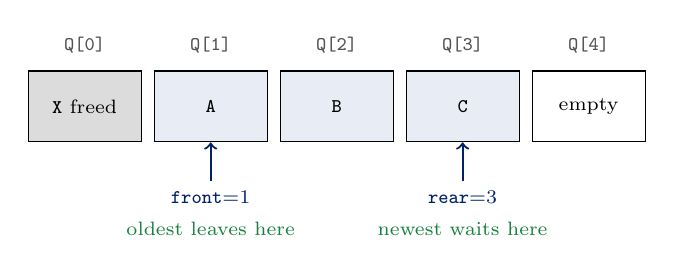
\begin{tikzpicture}[every node/.style={font=\scriptsize}]
    \node[draw, fill=neutral!20, minimum width=1.4cm, minimum height=0.9cm,
      text width=1.2cm, align=center] (q0) at (0, 0) {\texttt{X} freed};
    \node[draw, fill=light-bg, minimum width=1.4cm, minimum height=0.9cm,
      text width=1.2cm, align=center] (q1) at (1.6, 0) {\texttt{A}};
    \node[draw, fill=light-bg, minimum width=1.4cm, minimum height=0.9cm,
      text width=1.2cm, align=center] (q2) at (3.2, 0) {\texttt{B}};
    \node[draw, fill=light-bg, minimum width=1.4cm, minimum height=0.9cm,
      text width=1.2cm, align=center] (q3) at (4.8, 0) {\texttt{C}};
    \node[draw, fill=white, minimum width=1.4cm, minimum height=0.9cm,
      text width=1.2cm, align=center] (q4) at (6.4, 0) {empty};
    \node[text=neutral] at (0, 0.78) {\texttt{Q[0]}};
    \node[text=neutral] at (1.6, 0.78) {\texttt{Q[1]}};
    \node[text=neutral] at (3.2, 0.78) {\texttt{Q[2]}};
    \node[text=neutral] at (4.8, 0.78) {\texttt{Q[3]}};
    \node[text=neutral] at (6.4, 0.78) {\texttt{Q[4]}};
    \node[text=primary-blue] (flab) at (1.6, -1.15) {\texttt{front}=1};
    \draw[->, thick, color=primary-blue] (flab.north) -- (q1.south);
    \node[text=primary-blue] (rlab) at (4.8, -1.15) {\texttt{rear}=3};
    \draw[->, thick, color=primary-blue] (rlab.north) -- (q3.south);
    \node[text=positive] at (1.6, -1.55) {oldest leaves here};
    \node[text=positive] at (4.8, -1.55) {newest waits here};
  \end{tikzpicture}
  \caption{Linear queue: \texttt{X} was dequeued and its slot sits empty while \texttt{front} marches away from it. The queue holds 3 items but owns 5 slots.}
  \label{fig:linear}
\end{figure}

\begin{example}[Worked trace: enqueue, enqueue, dequeue]
Start with \texttt{front} $= 0$, \texttt{rear} $= -1$, empty. \texttt{enqueue(A)}: \texttt{rear} becomes 0, \texttt{Q[0]} $=$ \texttt{A}; state \texttt{[A]}, \texttt{front} $= 0$, \texttt{rear} $= 0$. \texttt{enqueue(B)}: \texttt{rear} becomes 1; state \texttt{[A B]}, \texttt{front} $= 0$, \texttt{rear} $= 1$. \texttt{enqueue(C)}: \texttt{rear} becomes 2; state \texttt{[A B C]}, \texttt{front} $= 0$, \texttt{rear} $= 2$. \texttt{dequeue} returns \texttt{Q[front]} \emph{before} the increment --- that ordering is load-bearing, because off-by-one here returns the wrong job --- so it returns \texttt{A} and \texttt{front} becomes 1; state \texttt{[B C]}, \texttt{front} $= 1$, \texttt{rear} $= 2$. \texttt{enqueue(D)}: \texttt{rear} becomes 3; state \texttt{[B C D]}, \texttt{front} $= 1$, \texttt{rear} $= 3$. After five operations the live items sit at indices 1--3; index 0 is dead space the implementation cannot reuse.
\end{example}

\subsection{The false-full trap}

Keep dequeuing and enqueuing: \texttt{front} and \texttt{rear} both drift right until \texttt{rear} $= n - 1$ with live items fewer than $n$. The implementation reports \bad{full} --- but slots $0$ to \texttt{front}$-1$ stand empty. Overflow with free space: a false alarm. The naive fix (shift everything left on each dequeue) restores honesty at $O(n)$ worst case per dequeue --- paying linear time to defend a constant-time contract. The real fix, which is the next section: let the indices wrap around the end of the array instead of marching off it --- one modular addition, no shifting, $O(1)$ kept.

\begin{example}[Prediction check: capacity 4, \texttt{enqueue} A, B, C, D, then \texttt{dequeue} twice, then \texttt{enqueue} E]
Of A: index 0 (dead slot reused); B: index 4 (overflow!); C: index 2 --- the answer the first-attempt code actually produces is B. Trace \texttt{front}/\texttt{rear} as numbers, not pictures. After four enqueues \texttt{front} $= 0$, \texttt{rear} $= 3$. Two dequeues move \texttt{front} to 2 (returning \texttt{A}, then \texttt{B}). \texttt{enqueue(E)} sets \texttt{rear} $= 3 + 1 = 4$: past the end of a capacity-4 array. A claims the linear code looks left --- it never does, so it cannot reuse index 0. C mistakes the live count (3 items) for a slot number --- E does not take ``the third slot,'' it takes \texttt{rear} $+ 1$.
\end{example}

\section{Circular Queue: One Index Calculation Reclaims the Array}

\textbf{Read alongside:} Karumanchi, Ch.~5, pp.205--223 (PDF) --- wraparound arithmetic, the full/empty tests, and the array cost analysis.

\subsection{Wraparound arithmetic}

\begin{definitionbox}{Circular advance (the rule)}
Advance every index modulo the capacity: \key{\texttt{rear} $=$ (\texttt{rear} $+ 1) \bmod n$}, \key{\texttt{front} $=$ (\texttt{front} $+ 1) \bmod n$}. Index $n - 1$ is followed by index $0$ --- the array is used as a ring. (Karumanchi Ch.~5, pp.205--223 PDF) \cite{Karumanchi2017_data_structures_algorithms_made_easy}.
\end{definitionbox}

Concrete instance, exactly as the deck states it: capacity $8$, \texttt{rear} $= 7$ $\to$ next \texttt{rear} $= (7 + 1) \bmod 8 = 0$. The ``past the end'' slot is the freed slot at the start. Cost of the fix: one division remainder per operation --- still $O(1)$ worst case. No shifting, ever.

Figure~\ref{fig:ring} draws the ring the deck draws: capacity 8, five live items \texttt{B}--\texttt{F} at indices 1--5, \texttt{front} $= 1$, \texttt{rear} $= 5$, slots 6, 7, and 0 standing empty, slot $0$ already recycled once, with the dashed wraparound arc marking the $7 \to 0$ step. The next \texttt{enqueue} lands at index $6$.

\begin{figure}[h]
  \centering
  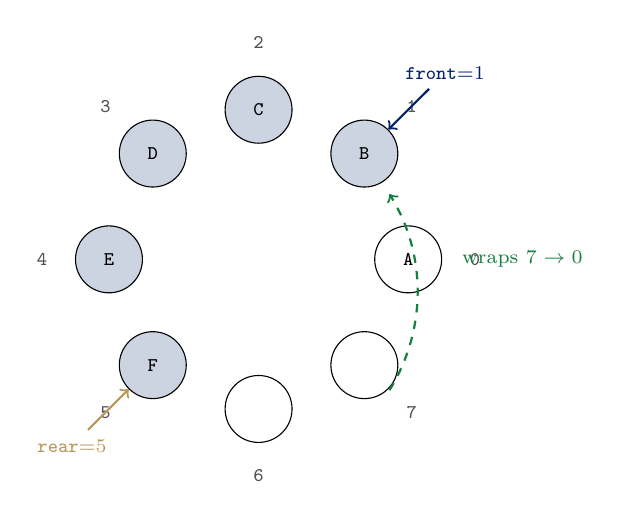
\begin{tikzpicture}[every node/.style={font=\scriptsize}]
    \node[draw, circle, fill=white, minimum width=0.85cm,
      minimum height=0.85cm] (s0) at (0:1.9) {\texttt{A}};
    \node[draw, circle, fill=primary-blue!20, minimum width=0.85cm,
      minimum height=0.85cm] (s1) at (45:1.9) {\texttt{B}};
    \node[draw, circle, fill=primary-blue!20, minimum width=0.85cm,
      minimum height=0.85cm] (s2) at (90:1.9) {\texttt{C}};
    \node[draw, circle, fill=primary-blue!20, minimum width=0.85cm,
      minimum height=0.85cm] (s3) at (135:1.9) {\texttt{D}};
    \node[draw, circle, fill=primary-blue!20, minimum width=0.85cm,
      minimum height=0.85cm] (s4) at (180:1.9) {\texttt{E}};
    \node[draw, circle, fill=primary-blue!20, minimum width=0.85cm,
      minimum height=0.85cm] (s5) at (225:1.9) {\texttt{F}};
    \node[draw, circle, fill=white, minimum width=0.85cm,
      minimum height=0.85cm] (s6) at (270:1.9) {\phantom{\texttt{G}}};
    \node[draw, circle, fill=white, minimum width=0.85cm,
      minimum height=0.85cm] (s7) at (315:1.9) {\phantom{\texttt{G}}};
    \node[text=neutral] at (0:2.75) {\texttt{0}};
    \node[text=neutral] at (45:2.75) {\texttt{1}};
    \node[text=neutral] at (90:2.75) {\texttt{2}};
    \node[text=neutral] at (135:2.75) {\texttt{3}};
    \node[text=neutral] at (180:2.75) {\texttt{4}};
    \node[text=neutral] at (225:2.75) {\texttt{5}};
    \node[text=neutral] at (270:2.75) {\texttt{6}};
    \node[text=neutral] at (315:2.75) {\texttt{7}};
    \node[text=primary-blue] (flab) at (45:3.35) {\texttt{front}=1};
    \draw[->, thick, color=primary-blue] (flab) -- (s1);
    \node[text=primary-gold] (rlab) at (225:3.35) {\texttt{rear}=5};
    \draw[->, thick, color=primary-gold] (rlab) -- (s5);
    \draw[->, thick, dashed, color=positive] (315:2.35) arc (-32:32:2.35);
    \node[text=positive] at (0:3.35) {wraps $7 \to 0$};
  \end{tikzpicture}
  \caption{Circular queue, capacity 8: five live items (\texttt{B}--\texttt{F}), \texttt{front} $= 1$, \texttt{rear} $= 5$; the next \texttt{enqueue} lands at index $6$, and slot $0$ was already recycled once.}
  \label{fig:ring}
\end{figure}

\subsection{Full or empty? They look identical}

With wraparound, \texttt{front} $=$ \texttt{rear} after the first enqueue \emph{and} when the ring is completely full --- one equality, two meanings. Two honest fixes, both stated exactly as the deck states them. \key{Fix A (count)}: keep \texttt{count} of live items; empty when \texttt{count} $= 0$, full when \texttt{count} $= n$ --- one extra integer. \key{Fix B (sacrificed slot)}: declare full when (\texttt{rear} $+ 1) \bmod n =$ \texttt{front}; the ring holds at most $n - 1$ items and one slot always stands empty. Course convention (Labs P5): use the \texttt{count} version --- it holds all $n$ items and its tests read plainly. Name your choice on paper --- examiners check the test, not the fashion.

\begin{example}[Worked trace: wrapping around (capacity 4, count version)]
\texttt{enq A, enq B, enq C}: \texttt{front} $= 0$, \texttt{rear} $= 2$, \texttt{count} $= 3$. \texttt{deq} $\to$ A, \texttt{deq} $\to$ B: each dequeue advances \texttt{front} modularly ($0 \to 1 \to 2$) and decrements the count; now \texttt{front} $= 2$, \texttt{rear} $= 2$, \texttt{count} $= 1$ (only \texttt{C} alive). \texttt{enq D}: \texttt{rear} $= (2+1) \bmod 4 = 3$; \texttt{front} $= 2$, \texttt{rear} $= 3$, \texttt{count} $= 2$. \texttt{enq E}: \texttt{rear} $= (3+1) \bmod 4 = 0$ --- the first wrap; \texttt{front} $= 2$, \texttt{rear} $= 0$, \texttt{count} $= 3$. \texttt{enq F}: \texttt{rear} $= (0+1) \bmod 4 = 1$ --- the second wrap; \texttt{front} $= 2$, \texttt{rear} $= 1$, \texttt{count} $= 4 =$ full. Watch \texttt{rear} walk $2 \to 3 \to 0 \to 1$: the wrap steps are where the linear code died, and the modular code does not even pause. The full test fires honestly: \texttt{count} $= 4 = n$ with every slot genuinely occupied.
\end{example}

Cost and code shape (Lab P5), in Week~2's shape: \texttt{enqueue}, \texttt{dequeue}, \texttt{front} --- each one array access plus one $\bmod$ --- $O(1)$ worst case, $O(1)$ auxiliary space beyond the $n$-slot array ($n$ = capacity here). The ring is the week's load-bearing idea: the same wraparound serves keyboard buffers, streaming windows, and Week~12's BFS frontier. Lab P5 implements exactly this trace: circular \texttt{enqueue} / \texttt{dequeue} / display with the full and empty tests above. The habit: name the operation (index advance), give the bound ($O(1)$), state the case (worst). ``Circular is $O(1)$'' without the case is half an answer.

\section{Double-Ended Queue: Both Ends Open}

\textbf{Read alongside:} Karumanchi, Ch.~5, pp.205--223 (PDF) --- the deque and its restricted variants (standard treatment for the naming).

\begin{definitionbox}{Deque}
A \key{deque} (``deck'') allows \texttt{enqueue} and \texttt{dequeue} at \emph{both} ends: \texttt{enqueueFront}, \texttt{enqueueRear}, \texttt{dequeueFront}, \texttt{dequeueRear}. A queue is a deque with two of the four operations switched off. (Karumanchi Ch.~5, pp.205--223 PDF; standard treatment) \cite{Karumanchi2017_data_structures_algorithms_made_easy}.
\end{definitionbox}

Motivation, exactly as the deck states it: an undo history takes new states at the rear but drops the \emph{oldest} states from the front when full --- one structure, both ends working. Array version: a circular ring with \texttt{front} allowed to step \emph{backwards}: \texttt{front} $=$ (\texttt{front} $- 1 + n) \bmod n$. The ring wraps underneath exactly as in the previous section; the new freedom is that \texttt{front} steps either direction, and so does \texttt{rear}.

\begin{figure}[h]
  \centering
  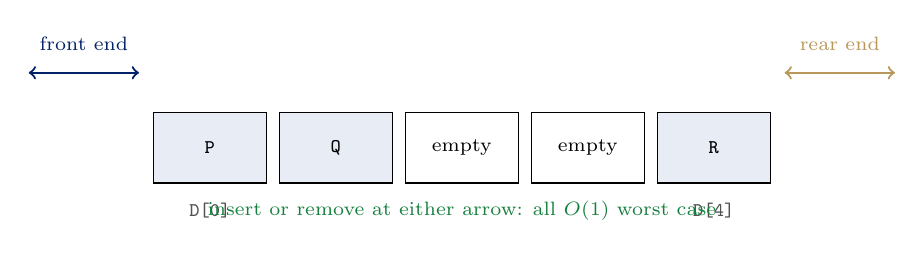
\begin{tikzpicture}[every node/.style={font=\scriptsize}]
    \node[draw, fill=light-bg, minimum width=1.4cm, minimum height=0.9cm,
      text width=1.2cm, align=center] (d0) at (0, 0) {\texttt{P}};
    \node[draw, fill=light-bg, minimum width=1.4cm, minimum height=0.9cm,
      text width=1.2cm, align=center] (d1) at (1.6, 0) {\texttt{Q}};
    \node[draw, fill=white, minimum width=1.4cm, minimum height=0.9cm,
      text width=1.2cm, align=center] (d2) at (3.2, 0) {empty};
    \node[draw, fill=white, minimum width=1.4cm, minimum height=0.9cm,
      text width=1.2cm, align=center] (d3) at (4.8, 0) {empty};
    \node[draw, fill=light-bg, minimum width=1.4cm, minimum height=0.9cm,
      text width=1.2cm, align=center] (d4) at (6.4, 0) {\texttt{R}};
    \node[text=neutral] at (0, -0.80) {\texttt{D[0]}};
    \node[text=neutral] at (6.4, -0.80) {\texttt{D[4]}};
    \draw[<->, thick, color=primary-blue] (-2.3, 0.95) -- (-0.9, 0.95);
    \node[text=primary-blue] at (-1.6, 1.32) {front end};
    \draw[<->, thick, color=primary-gold] (7.3, 0.95) -- (8.7, 0.95);
    \node[text=primary-gold] at (8.0, 1.32) {rear end};
    \node[text=positive] at (3.2, -0.80)
      {insert or remove at either arrow: all $O(1)$ worst case};
  \end{tikzpicture}
  \caption{Deque strip: insert or remove at either arrow, all $O(1)$ worst case. The ring wraps underneath as in Fig.~5.2; the new freedom is bidirectional stepping.}
  \label{fig:deque}
\end{figure}

\begin{example}[Worked deque state and its restricted cousins]
Start empty (capacity 5): \texttt{enqueueRear(Q)}, \texttt{enqueueRear(R)} $\to$ rear grows right; \texttt{enqueueFront(P)} $\to$ front steps left with wraparound. The state drawn in Fig.~5.3 is \texttt{[P Q \_ \_ R]} with both arrows live. Two restricted cousins, named exactly as the deck names them. \key{Input-restricted deque}: insert at one end only, remove at either --- models a priority lane that admits newcomers singly. \key{Output-restricted deque}: insert at either end, remove at one end only --- models a pipeline with a single outlet. Exam note, verbatim: if a question says ``insert at rear, delete at both ends'': that is the input-restricted deque. Name it, then trace it --- the name earns the first mark, the trace the rest.
\end{example}

\section{Priority Queue Using Arrays: Urgency Instead of Arrival}

\textbf{Read alongside:} Karumanchi, Ch.~7, pp.369--408 (PDF) --- the Priority Queue ADT and its array designs; Sedgewick \& Wayne, Sec.~2.4, p.~308 --- priority queues.

When arrival order is the wrong order: the OS scheduler holds processes \texttt{(job, priority)} --- a system interrupt (priority 0) must run before a background backup (priority 9), however late it arrived. FIFO would run the backup first. Hospital triage, printer ``urgent'' flags, Dijkstra's frontier (Week~12): every one ranks by \key{priority}, not by arrival time. Syllabus constraint, stated plainly: implement it \emph{using arrays} --- no heaps yet (heaps arrive with trees in Week~11). Two honest array designs, opposite bills.

\begin{definitionbox}{Priority queue}
A \key{priority queue} returns the minimum (or maximum) priority item first. Insert is \texttt{enqueue} with a priority; removal is \texttt{deleteMin} (or \texttt{deleteMax}). (Karumanchi Ch.~7, pp.369--408 PDF; Sedgewick Sec.~2.4, p.~308) \cite{Karumanchi2017_data_structures_algorithms_made_easy,Sedgewick2011_algorithms}.
\end{definitionbox}

\begin{center}
{\footnotesize
\begin{tabular}{lll}
  \toprule
  \textbf{design} & \textbf{insert} & \textbf{\texttt{deleteMin}} \\
  \midrule
  Unordered (append) & $O(1)$ worst case & scan all $n$: $O(n)$ worst \\
  Ordered (sorted) & shift room: $O(n)$ worst & read off end: $O(1)$ worst \\
  \bottomrule
\end{tabular}}
\end{center}

No free lunch with arrays: one end of the trade is always linear. (Week~11's heap makes both $O(\log n)$ --- the reason heaps exist.) Choose by workload: many inserts, few removals $\to$ unordered; removals dominate $\to$ ordered.

\begin{figure}[h]
  \centering
  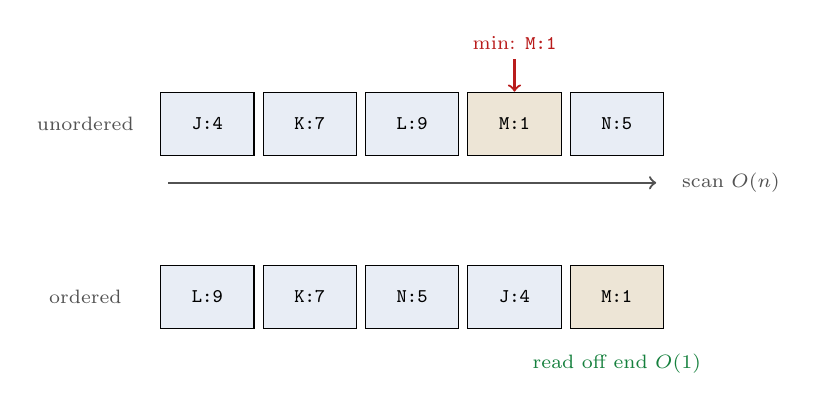
\begin{tikzpicture}[every node/.style={font=\scriptsize}]
    \node[text=neutral] at (-2.85, 1.1) {unordered};
    \node[draw, minimum width=1.15cm, minimum height=0.8cm, fill=light-bg,
      text width=0.95cm, align=center] (u0) at (-1.3, 1.1) {\texttt{J:4}};
    \node[draw, minimum width=1.15cm, minimum height=0.8cm, fill=light-bg,
      text width=0.95cm, align=center] (u1) at (0, 1.1) {\texttt{K:7}};
    \node[draw, minimum width=1.15cm, minimum height=0.8cm, fill=light-bg,
      text width=0.95cm, align=center] (u2) at (1.3, 1.1) {\texttt{L:9}};
    \node[draw, minimum width=1.15cm, minimum height=0.8cm,
      fill=primary-gold!25, text width=0.95cm, align=center] (u3) at (2.6, 1.1) {\texttt{M:1}};
    \node[draw, minimum width=1.15cm, minimum height=0.8cm, fill=light-bg,
      text width=0.95cm, align=center] (u4) at (3.9, 1.1) {\texttt{N:5}};
    \draw[->, thick, color=neutral] (-1.8, 0.35) -- (4.4, 0.35);
    \node[text=neutral] at (5.35, 0.35) {scan $O(n)$};
    \node[text=negative] at (2.6, 2.12) {min: \texttt{M:1}};
    \draw[->, thick, color=negative] (2.6, 1.92) -- (u3.north);
    \node[text=neutral] at (-2.85, -1.1) {ordered};
    \node[draw, minimum width=1.15cm, minimum height=0.8cm, fill=light-bg,
      text width=0.95cm, align=center] (s0) at (-1.3, -1.1) {\texttt{L:9}};
    \node[draw, minimum width=1.15cm, minimum height=0.8cm, fill=light-bg,
      text width=0.95cm, align=center] (s1) at (0, -1.1) {\texttt{K:7}};
    \node[draw, minimum width=1.15cm, minimum height=0.8cm, fill=light-bg,
      text width=0.95cm, align=center] (s2) at (1.3, -1.1) {\texttt{N:5}};
    \node[draw, minimum width=1.15cm, minimum height=0.8cm, fill=light-bg,
      text width=0.95cm, align=center] (s3) at (2.6, -1.1) {\texttt{J:4}};
    \node[draw, minimum width=1.15cm, minimum height=0.8cm,
      fill=primary-gold!25, text width=0.95cm, align=center] (s4) at (3.9, -1.1) {\texttt{M:1}};
    \node[text=positive] at (3.9, -1.95) {read off end $O(1)$};
  \end{tikzpicture}
  \caption{Priority queue on arrays: unordered row scanned at $O(n)$ worst case to find \texttt{M:1}; ordered row read off the end at $O(1)$ worst case.}
  \label{fig:prio}
\end{figure}

\begin{example}[Trace \texttt{deleteMin} on the drawn queues]
Unordered row holds \texttt{J:4, K:7, L:9, M:1, N:5}. Scan all five priorities, return \texttt{M:1}, close the gap by shifting (unordered) --- that scan is the $O(n)$ worst-case bill. Ordered row holds the same five jobs sorted (\texttt{L:9, K:7, N:5, J:4, M:1}); take the end slot --- the $O(1)$ worst-case read. Lab P6 implements the unordered version. The price was paid at insertion instead: keeping the row sorted cost a shift per insert ($O(n)$ worst case).
\end{example}

\begin{example}[Prediction check: 1\,000 inserts then 3 removals, or 3 inserts then 1\,000 removals?]
Of A: ordered for both; B: unordered, then ordered; C: unordered for both --- the answer is B. Price the workload, not the structure: count which operation runs hot, then read the table. Many inserts with few removals: pay the linear bill on the rare operation (the scan) and keep the frequent one constant --- unordered. Removals dominant: pay at insertion and keep each removal constant --- ordered. A sorts once up front even when removals are rare (paying $O(n)$ per insert to save three scans); C scans a thousand times when one sort would have served.
\end{example}

\section{Unit-I Map, Mistakes, Summary, and What Comes Next}

\textbf{Read alongside:} Weeks~1--4 decks for the traced tables; no new anchor reading in this section.

Unit I in one map (Class Test 1), reproduced exactly as the deck tabulates it:

\begin{center}
{\footnotesize
\begin{tabular}{lll}
  \toprule
  \textbf{week} & \textbf{contract} & \textbf{load-bearing skill} \\
  \midrule
  1 & ADT; \texttt{malloc}/\texttt{free}, \texttt{NULL} & ownership tracing \\
  2 & $T(n)$, $O/\Omega/\Theta$, best/worst/average & price every claim \\
  3 & Stack ADT; \texttt{top} $= -1$ empty; $O(1)$ & bracket check, postfix eval \\
  4 & Notations; conversion; recursion; Hanoi $\Theta(2^{n})$ & stack traces \\
  5 & Queue; \texttt{front}/\texttt{rear}; $\bmod$ ring & buffer traces (today) \\
  \bottomrule
\end{tabular}}
\end{center}

The test rewards the course habit: name the structure, trace it line by line, state operation $+$ bound $+$ case. Every structure so far lives in an array; Week~6 asks what pointers buy us instead.

Three common mistakes across all of Unit I, stated exactly as the deck states them. \bad{Confusing the case with the bound} --- ``best case $O(n)$'' mixes the input (case) with the growth class (bound). Say ``best case $\Theta(1)$, worst case $\Theta(n)$'' with the operation named. \bad{Testing full as \texttt{front} $=$ \texttt{rear}} --- that test also fires on empty. Use \texttt{count} ($0$ vs.\ $n$) or sacrifice a slot, and write the test down before the code. \bad{Forgetting direction} --- stacks pop the young end, queues the old end, deques either end, priority queues the urgent end. State the removal rule first; the code follows it. How to revise: re-trace one table per week (Weeks 3, 4, and today's two) with a covered answer column --- the test is traces, not definitions.

In summary: \key{Queue} --- \texttt{enqueue} at \texttt{rear}, \texttt{dequeue} from \texttt{front}; $O(1)$ worst case each; the linear array dies of false fullness. \key{Circular queue} --- $(\cdot + 1) \bmod n$ recycling; full vs.\ empty by \texttt{count} or sacrificed slot; Lab P5. \key{Deque} --- four operations, both ends, backward-stepping \texttt{front}; restricted cousins name which end is closed. \key{Priority queue on arrays} --- unordered ($O(1)$ insert, $O(n)$ \texttt{deleteMin}) vs.\ ordered (flipped); Lab P6; heaps in Week~11. Next week: linked lists --- what changes when nodes carry their own links instead of sitting in numbered slots --- and the queue reborn on pointers (Week~7).

\begin{example}[Before-you-go predictions (Class Test 1 warm-up), with the deck's answers]
Answer from the algorithms, then check in the labs (P5, P6). (1) Capacity 5, \texttt{front} $= 3$, \texttt{rear} $= 1$, \texttt{count} $= 4$: full or not? After one \texttt{dequeue} and one \texttt{enqueue}, what are the three values? Not full ($4 < 5$); then \texttt{front} $= 4$, \texttt{rear} $= 2$, \texttt{count} $= 4$ --- the dequeue advances \texttt{front} $(3+1) \bmod 5 = 4$ with count $3$, and the enqueue advances \texttt{rear} $(1+1) \bmod 5 = 2$ with count back to $4$. (2) Name the deque variant: insert rear-only, remove either end. Input-restricted deque. (3) Unordered priority queue holds \texttt{A:3, B:1, C:2}: \texttt{deleteMin} returns what, and what does it cost worst case? Returns \texttt{B:1} at $O(n)$ worst case --- the scan touches all three.
\end{example}

\subsection*{Exercises}

Answer from the algorithms, then check in the labs: circular traces are Lab P5, the unordered priority queue is Lab P6.
\begin{enumerate}
  \item Linear queue, capacity 5, \texttt{front} $= 0$, \texttt{rear} $= -1$: run \texttt{enqueue(A)}, \texttt{enqueue(B)}, \texttt{dequeue}, \texttt{enqueue(C)}, \texttt{enqueue(D)}, \texttt{dequeue}. Give \texttt{front}, \texttt{rear}, and the live contents after each step, and name the dead slot(s).
  \item Circular queue (count version), capacity 4: start from \texttt{front} $= 0$, \texttt{rear} $= 3$, \texttt{count} $= 4$ (full). Run \texttt{dequeue}, \texttt{dequeue}, \texttt{enqueue(X)}, \texttt{enqueue(Y)}, \texttt{enqueue(Z)}. Give the three values after each step and show both wraparound computations.
  \item Capacity 6 (count version), \texttt{front} $= 5$, \texttt{rear} $= 4$, \texttt{count} $= 6$: is it full? After two dequeues and one enqueue, what are \texttt{front}, \texttt{rear}, \texttt{count}? (Genuinely new instance reusing the deck's modular rule.)
  \item Deque, capacity 5: \texttt{enqueueRear(A)}, \texttt{enqueueRear(B)}, \texttt{enqueueFront(C)}, \texttt{dequeueRear}, \texttt{enqueueFront(D)}. Give the live contents and state which restricted variant (if any) this operation sequence stays inside.
  \item Unordered priority queue holds \texttt{P:5, Q:2, R:4}: \texttt{deleteMin} returns what at what worst-case cost? If instead 500 inserts precede 2 removals, which array design does the deck's workload rule pick, and why?
\end{enumerate}

\subsection*{Solutions}

\begingroup\small
\begin{enumerate}
  \item \textbf{\texttt{front} $= 2$, \texttt{rear} $= 3$, live \texttt{[C D]}; dead slot: index 0 (and index 1 after the second dequeue).} Trace: start (0, $-1$, empty). \texttt{enq A} $\to$ (0, 0, \texttt{[A]}). \texttt{enq B} $\to$ (0, 1, \texttt{[A B]}). \texttt{deq} $\to$ \texttt{A}, (1, 1, \texttt{[B]}); index 0 dead. \texttt{enq C} $\to$ (1, 2, \texttt{[B C]}). \texttt{enq D} $\to$ (1, 3, \texttt{[B C D]}). \texttt{deq} $\to$ \texttt{B}, (2, 3, \texttt{[C D]}); indices 0--1 dead and unrecoverable by the linear code.
  \item \textbf{Ends at \texttt{front} $= 2$, \texttt{rear} $= 2$, \texttt{count} $= 4$ (full again); wraps at the enqueues of X ($3 \to 0$) and Y ($0 \to 1$); Z refused.} Trace: start (0, 3, 4). \texttt{deq} $\to$ (1, 3, 3). \texttt{deq} $\to$ (2, 3, 2). \texttt{enq X}: \texttt{rear} $= (3+1) \bmod 4 = 0$ $\to$ (2, 0, 3). \texttt{enq Y}: \texttt{rear} $= (0+1) \bmod 4 = 1$ $\to$ (2, 1, 4). \texttt{enq Z}: refused --- \texttt{count} $= 4 = n$, full; the honest test blocks the write.
  \item \textbf{Full ($6 = n$). After the three operations: \texttt{front} $= 1$, \texttt{rear} $= 5$, \texttt{count} $= 5$.} Full test: \texttt{count} $= 6 = n$. Dequeue: \texttt{front} $= (5+1) \bmod 6 = 0$, count $5$. Dequeue: \texttt{front} $= (0+1) \bmod 6 = 1$, count $4$. Enqueue: \texttt{rear} $= (4+1) \bmod 6 = 5$, count $5$. Not full ($5 < 6$).
  \item \textbf{Live \texttt{[D C A]} (front to rear); the sequence is a full deque --- it uses both-end insertion, so it stays inside neither restricted variant.} Trace: \texttt{enqRear(A)} $\to$ \texttt{[A]}; \texttt{enqRear(B)} $\to$ \texttt{[A B]}; \texttt{enqFront(C)} $\to$ \texttt{[C A B]}; \texttt{deqRear} removes \texttt{B} $\to$ \texttt{[C A]}; \texttt{enqFront(D)} $\to$ \texttt{[D C A]}. Input-restricted allows insert at one end only and output-restricted allows remove at one end only --- this sequence inserts at both ends (\texttt{enqRear} and \texttt{enqFront}), so it needs the unrestricted deque.
  \item \textbf{Returns \texttt{Q:2} at $O(n)$ worst case; 500 inserts with 2 removals $\to$ unordered.} \texttt{deleteMin} scans all three priorities and returns the minimum \texttt{Q:2}; the scan is $O(n)$ worst case. Workload rule (deck's table): pay the linear bill on the rare operation --- with inserts hot and removals rare, keep insert $O(1)$ (unordered) and accept the $O(n)$ scan twice.
\end{enumerate}
\endgroup

\bibliography{../../Bibliography_base}
\bibliographystyle{plain}
\end{document}
